%%%%%%%%%%%%%%%%%%%%%%%%%%%%%%%%%%%%%%%%%%%%%%%%%%%%%%%%%%%
% --------------------------------------------------------
% Rho
% LaTeX Template
% Version 2.1.1 (01/09/2024)
%
% Authors: 
% Guillermo Jimenez (memo.notess1@gmail.com)
% Eduardo Gracidas (eduardo.gracidas29@gmail.com)
% 
% License:
% Creative Commons CC BY 4.0
% --------------------------------------------------------
%%%%%%%%%%%%%%%%%%%%%%%%%%%%%%%%%%%%%%%%%%%%%%%%%%%%%%%%%%%

\documentclass[9pt,a4paper,twoside]{rho-class/rho}
\usepackage[english]{babel}

%% Spanish babel recomendation
% \usepackage[spanish,es-nodecimaldot,es-noindentfirst]{babel}

\setbool{rho-abstract}{true} % Set false to hide the abstract
\setbool{corres-info}{true} % Set false to hide the corresponding author section

%----------------------------------------------------------
% TITLE
%----------------------------------------------------------

\journalname{Example Template}
\title{Template for preparing an academic article or lab report using the rho \LaTeX\ class in Overleaf}

%----------------------------------------------------------
% AUTHORS AND AFFILIATIONS
%----------------------------------------------------------

\author[1,$\dagger$]{Author One}
\author[2]{Author Two}
\author[3,$\dagger$]{Author Three}

%----------------------------------------------------------

\affil[1]{Affiliation of author one}
\affil[2]{Affiliation of author two}
\affil[3]{Affiliation of author three}
\affil[$\dagger$]{These authors contributed equally to this work}

%----------------------------------------------------------
% DATES
%----------------------------------------------------------

\dates{This manuscript was compile on September 1, 2024}

%----------------------------------------------------------
% FOOTER INFORMATION
%----------------------------------------------------------

\leadauthor{Author last name et al.}
\footinfo{Creative Commons CC BY 4.0}
\smalltitle{\LaTeX\ Template}
\institution{College name}
\theday{May 21, 2024} %\today

%----------------------------------------------------------
% ARTICLE INFORMATION
%----------------------------------------------------------

\corres{Provide the corresponding author information and publisher here.}
\email{example@organization.com.}
\doi{\url{https://www.doi.org/exampledoi/XXXXXXXXXX}}

\received{March 20, 2024}
\revised{April 16, 2024}
\accepted{April 20, 2024}
\published{May 21, 2024}

\license{Rho LaTeX Class \ccLogo\ This document is licensed under Creative Commons CC BY 4.0.}

%----------------------------------------------------------
% ABSTRACT
%----------------------------------------------------------

\begin{abstract}
    Welcome to rho ($\rho$) \LaTeX\ class for making academic articles and lab reports. In this example template, we will guide you through the process of using and customizing the document to your needs. For more information of this class check out the appendix section. There, you will find codes that define key aspects of the template, allowing you to explore and modify them. If you do not need the abstract set \textit{false} to rho-abstract. It is worth to mention that this template is inspired by an earlier work, the \href{https://es.overleaf.com/latex/templates/tau-class-lab-report-template/chhshmhxstsq}{tau} \LaTeX\ class, designed with academic intentions.
\end{abstract}

%----------------------------------------------------------

\keywords{keyword 1, keyword 2, keyword 3, keyword 4, keyword 5}

%----------------------------------------------------------

\begin{document}
	
    \maketitle
    \thispagestyle{firststyle}
    % \tableofcontents
    \linenumbers

%----------------------------------------------------------

\section{Introduction}

    \rhostart{W}elcome to \textit{rho class} template for preparing your academic article or lab report. Throughout this guide, we will show you how to use this template and how to make modifications to this class. 
    
    This class includes the following files placed in the ‘rho-class’ folder: rho.cls, rhoenvs.sty, rhobabel.sty and README.md.

    \section{Casos reales}

    \subsection{Detección de abuso y fraude en servicios de streaming mediante Machine Learning con reconocimiento heurístico}
        La Plataforma de streaming Netflix desarrollo un framework para la detección de fraudes en su aplicación empleando algoritmos heurísticos desarrollados en la compañía y Machine Learning (ML), usando diferentes fuentes de datos como la trazabilidad de los usuarios, conexiones, contenido visualizado, ubicaciones, entre otros. Los autores Esmaeilzadeh et al. (2022) \cite{FraudDetection} , expresan en su artículo que desarrollar un modelo ML para la detección de anomalías en el contexto de su aplicación implica muchos retos, entre ellos están, el análisis en tiempo real que puede llegar a ser costoso en términos de infraestructura y poca escalable, la definición de anomalía depende del contexto de negocio y aplicación y la cantidad de datos para alimentar al modelo, ya que al tratarse de casos no recurrentes se presenta una disparidad en la cantidad de datos. Debido a estas razones los autores plantean las siguientes soluciones. Primero, una solución basada en reglas que permita identificar irregularidades tomando como base el conocimiento y experiencia a de los expertos de negocio, brindando características esenciales y contexto sobre los incidentes que permitan elaborar algoritmos heurísticos. Segundo, aplicar otra solución basado en modelo que permita identificar los casos anormales en la plataforma de forma automática. Para ejecutar este marco de trabajo primero se separaron en tres tipos de fraude, de cuentas, servicios y contenido, entonces la primera solución planteada complementa a la segunda, ya que ayuda a etiquetar y limpiar los datos que ingesta a la segunda solución, con la finalidad de identificar cual es el fraude que mas se comete en la aplicación y poder identificar la cuenta asociada al cliente que infringe las políticas de la aplicación. Por último, con algoritmos heurísticos desarrollados con base a la experiencia y conocimiento de los expertos, complementa un modelo ML incrementando su precisión hasta en un 86\% en el análisis de fraude en tiempo real.

    \subsection{Uso de Machine Learning para predecir el proximo archivo}
        Un segundo caso de éxito lo aplica la empresa de servicio de almacenamiento en la nube Dropbox, en su artículo de ingeniería el autor Kumar (2019) \cite{PredictFile} presenta como una funcionalidad de predicción de archivos que parece simple para el usuario tiene una gran complejidad por detrás, esto se debe a que para poder desarrollarlo realizaron algunos algoritmos heurísticos tomando como punto de inicio variables como la frecuencia con la que se accede a un archivo y el acceso reciente, sobre esto implementaron los algoritmos para obtener la probabilidad de cuál sería el próximo archivo que el usuario necesitaría, sin embargo, algunos obstáculos en ciertos escenario y el incremento en la complejidad computacional es que optaron por construir un primer modelo de Machine Learning que pueda analizar el comportamiento del usuario sobre los archivos que crea y modifica dentro de la aplicación.

    \subsection{Conclusion}
        De los casos de éxito se llega a la conclusión que se puede aplicar heurística en diferente entornos y problemas, mediante el desarrollo de algoritmos heurísticos se puede desarrollar soluciones escalables y eficientes, a modo de ejemplo el caso de Netflix que mediante estos algoritmos pudo entrenar un modelo de ML mucho mas grande y solucionar el problema de fraude en su plataforma, también el caso de Dropbox que pudo desarrollar una funcionalidad para el usuario final brindando facilidad en la navegación entre los archivos de su plataforma.

\section{Other elements}

    \subsection{Lettrine}
    
        The \verb*|\rhostart{}| command provides a personalized lettrine for the beginning of a paragraph as shown in this document example.

    \subsection{Line numbering}

        By implementing the \textit{lineno} package, the line numbering of the document can be placed with the command \verb|\linenumbers|. 
		
        I recommend placing the command after the table of contents for a better appearance (comment or delete if not required).

\section{Equation}

    Equation \ref{ec:equation}, shows the Schrödinger equation as an example. 
        \begin{equation} \label{ec:equation}
            \frac{\hbar^2}{2m}\nabla^2\Psi + V(\mathbf{r})\Psi = -i\hbar \frac{\partial\Psi}{\partial t}
        \end{equation} 
    The \textit{amssymb} package was not necessary to include, because stix2 font incorporates mathematical symbols for writing quality equations. In case you choose another font, uncomment the package in \textit{rho class}.

    In case you want to change the values that adjust the spacing above and below in the equations, go to \textit{rho-class/rho.cls/math packages} section and play with \verb|\setlength{\eqskip}{8pt}| value until the preferred spacing is set.

\section{Rho packages}

    \subsection{Rhoenvs}
    
        This template has its own environment package \textit{rhoenvs.sty} designed to enhance the presentation of information within documents. Among these custom environments are \textit{rhoenv}, \textit{info} and \textit{note}.
    
        There are two environments which have a predefined title. These can be included by the command \verb|\begin{note}| and \verb|\begin{info}|. All the environments have the same style.
    	
        An example using the rho environment is shown below.
    
        \begin{rhoenv}[frametitle=Environment with custom title]
            Hello! I am an example of the \textit{rhoenv} included in rhoenvs \LaTeX\ package. Here you can include relevant information or notes about your work. You can modify my title directly in the code.
        \end{rhoenv}
    
        Rhoenv is the only environment that you can customize its title. On the other hand, \textit{info} and \textit{note} adapt their title to Spanish automatically when the language package is defined.

    \subsection{Rhobabel}

        In this new version, we have included a package called \textit{rhobabel}, which have all the commands that automatically translate from English to Spanish when this language package is defined. 
        
        By default, rho displays its content in English. However, at the beginning of the document you will find a recommendation when writing in Spanish. 
		
        \textit{Note:} You may modify this package if you want to use other language than English or Spanish. This will make easier to translate the document without having to modify the class document.

\section{Figures and tables}

    \subsection{Sample figure}

        Figure \ref{fig:figure} shows an example figure.
        
            \begin{figure}[H]
                \centering
                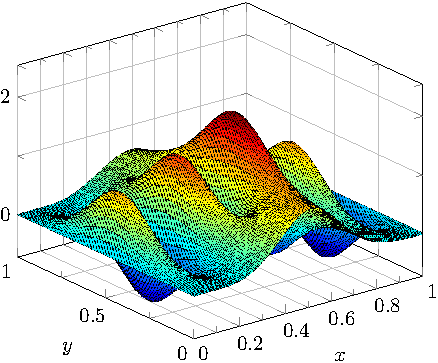
\includegraphics[width=0.71\columnwidth]{Example.pdf}
                \caption{Example figure obtained from PGFPlots \cite{PFGPlots}.}
                \label{fig:figure}
            \end{figure}

    \subsection{Sample double figure}

        Figure \ref{fig:examplefloat} shows an example of a two-picture floating figure that covers the width of the page. It can be positioned at the top or bottom of the page. The space between the figures can also be changed using the \verb|\hspace{Xpt}| command.

        \begin{figure*}[t!] % t for position at the top of the current page; b for position at the bottom of the current page
            \centering
                \begin{subfigure}[b]{0.38\linewidth} % Fig (a)
                    \includegraphics[width=\linewidth]{Example2.pdf}
                    \caption{Example left figure.}
                    \label{fig:figa}
                \end{subfigure}
            \hspace{15pt}   % Space between the figures
                \begin{subfigure}[b]{0.38\linewidth} % Fig (b)
                    \centering
                    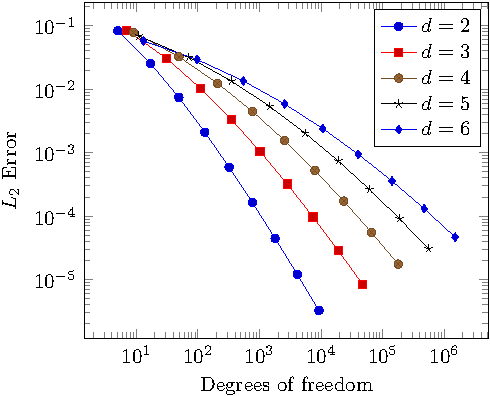
\includegraphics[width=\linewidth]{example2.pdf}
                    \caption{Example right figure.}
                    \label{fig:figb}
                \end{subfigure}
            \caption{Example figure that covers the width of the page obtained from PGFPlots \cite{PFGPlots}.}
            \label{fig:examplefloat}
        \end{figure*}

    \subsection{Sample table}

        In the same way as the figures, you can place tables in one or two columns, depending on the length of the table.

        Table \ref{tab:table}, shows an example table that covers the width of the page positioned at the bottom of a new page.

        \begin{table*}[pb]
            \RaggedRight
            \caption{Table example that covers the width of the page.}
            \label{tab:table}
                \begin{tabular}{lllp{12.2cm}}
                    \toprule
                    \textbf{Day} & \textbf{Min Temp} & \textbf{Max Temp} & \textbf{Summary} \\ 
                    \midrule
                    Monday & 11\textdegree C & 22\textdegree C & A clear day with lots of sunshine.  Strong breeze will bring down the temperatures. \\
                    Tuesday & 9\textdegree C & 19\textdegree C & Cloudy with rain, across many northern regions. \\
                    Wednesday & 10\textdegree C & 21\textdegree C & Rain will still linger for the morning. 
                    Conditions will improve by early afternoon and continue 
                    throughout the evening.\\
                    \bottomrule
                \end{tabular}
                
            \tabletext{Note: Obtained from \LaTeX\ tables \cite{projects-2023}.}
            
        \end{table*}

\section{Codes}

    This class\footnote{Hello there! I am a footnote :)} includes the \textit{listings} package, which offers customized features for adding codes specially for C, C++, \LaTeX\ and Matlab. You can customize the format in \textit{rho class} file.

    \nolinenumbers
    \lstinputlisting[caption=Example of matlab code., label={lst:listing-Mat}, language=Matlab]{example.m}
    \linenumbers
    
    If line numbering is enabled, we recommend placing the command \verb|\nolinenumbers| at the beginning and \verb|\linenumbers| at the end of the code. 
    
    This will temporarily remove line numbering and the code will look better.

\section*{Unnumbered section} \label{sec:unsec}

    If a unnumbered section is declared, a square appears followed by the section name. This style is characteristic of this class and is only for first level sections.

    Since this affects the title of the table of contents and references, you can make a modification in \textit{rho-class/rho.cls/section style} to remove the square. See appendix for more information.

\section{Table of contents}

    The ToC provides a preview of the content and its location in the document. Uncomment the command \verb|\tableofcontents| to display it. Remember that unnumbered sections will not appear in the ToC, however, you can place them manually with the command \verb|\addcontentsline{toc}{section}{section name}|.

    See the appendix section for more information. There, you will find recommended modifications to adjust the table of contents when unnumbered sections are defined.

\section{Reference style}

    The default formatting for references follows the IEEE style. At the end of the document, you will find an example of the default reference formatting.

    You can modify the style of your references, for that, go to \textit{rho-class/rho.cls/biblatex}. See appendix for more information.

\section{Appendix}

    \subsection{Unnumbered sections}

        As mentioned in section \ref{sec:unsec}, when placing a first level section without number a square appears followed by the section name. In case you do not require this extra detail, you can make the following modification.

\nolinenumbers
\begin{lstlisting}[language=TeX, caption=Alternative unnumbered section.]
\titleformat{name=\section,numberless}[block]
    {\color{rhocolor}\sffamily\large\bfseries}
    {}
    {0em}
    {#1}
    []
\end{lstlisting}
\linenumbers

        You can change to this code in \textit{rho-class/rho.cls/section style}. Once the document is recompiled, this square will disappear. 

        Remember that this code affects the ToC and references title. To show rho class functionalities, this option is enabled by default.

    \subsection{Table of contents}
    
        In case you have chosen the unnumbered sections and you want to add the ToC, you can do the following to adjust the content.

\nolinenumbers
\begin{lstlisting}[language=TeX, caption=ToC when unnumbered section is chosen.]
\setlength\tocsep{0pc}

\titlecontents{section}[\tocsep]
    {\addvspace{4pt}\sffamily\selectfont\bfseries}
    {\contentslabel[\thecontentslabel]{\tocsep}}
    {}
    {\hfill\thecontentspage}
    []

\titlecontents{subsection}[1pc]
    {\addvspace{4pt}\small\sffamily\selectfont}
    {\contentslabel[\thecontentslabel]{\tocsep}}
    {}
    {\ \titlerule*[.5pc]{.}\ \thecontentspage}
    []

\titlecontents*{subsubsection}[1pc]
    {\footnotesize\sffamily\selectfont}
    {}
    {}
    {}
    [\ \textbullet\ ]
\end{lstlisting}
\linenumbers

        As you can see, the value of \verb|\tocsep| was changed to 0pc for the sections. For subsections and subsubsections the value was changed to 1pc.

        By making this small modification, the contents of the ToC will look more organized.

        If you use numbered sections, you do not need to make this modifications, unless you prefer other values.

    \subsection{References and paths}

        In case you require another reference style, you can go to \textit{rho-class/rho.cls/biblatex} and modify the following. 

\nolinenumbers
\begin{lstlisting}[language=TeX, caption=Reference code.]
\usepackage[
    backend=biber,
    style=ieee,
    sorting=ynt
]{biblatex}
\end{lstlisting}
\linenumbers

        By default, rho class has its own .bib for this example, if you want to name your own bib file, change the following path.

\nolinenumbers
\begin{lstlisting}[language=TeX]
\addbibresource{rho.bib}
\end{lstlisting}
\linenumbers

    \subsection{Info environment}

        We will show an example of the info environment declared in the ‘rhoenvs.sty’ package. Remember that \textit{info} and \textit{note} are the only packages that translate their title (English or Spanish).

        \begin{info}
            Small example of info environment.
        \end{info}

\section{Supporting}

    Did you like this class document? Check out \href{https://www.overleaf.com/latex/templates/tau-class-lab-report-template/chhshmhxstsq}{tau class} designed for your lab reports.

    \subsection*{Any contributions are welcome!}
    
        Coffee keeps us awake and helps us create better \LaTeX\ templates. If you wish to support our work, you can do so through PayPal:\\
        \url{https://www.paypal.me/GuillermoJimeenez}.
        
        \begin{center}
            Enjoy writing with rho \LaTeX\ class\hspace{5pt}\faChessKnight 
        \end{center}

\section{Contact us}

    You can contact us through these methods.\\
    
    \noindent\faWix\hspace{5pt}\href{https://memonotess1.wixsite.com/memonotess}{https://memonotess1.wixsite.com/memonotess} \\
    \faEnvelope[regular]\hspace{7pt}memo.notess1@gmail.com \\
    \faEnvelope[regular]\hspace{7pt}eduardo.gracidas29@gmail.com \\
    \faInstagram\hspace{8pt}memo.notess
        
%----------------------------------------------------------

\printbibliography

%----------------------------------------------------------

\end{document}